\section{AlarmClockWeb}
Nastavení budicích časů z rozhraní na LCD budíku je poměrně pohodlné
a přímočaré, pokud ale uživatel potřebuje udělat rozsáhlejší úpravy, může
preferovat konfiguraci z počítače či mobilního telefonu.
Z tohoto důvodu byla vytvořena jednoduchá webová stránka sloužící k tomuto
účelu. Stránka je tvořena skriptem v jazyce PHP, který se připojí na MQTT API
budíku a z dat z něj získaných vygeneruje obsah webové stránky ve značkovacím
jazyce HTML. Tato stránka obsahuje formulář, jehož odesláním je možné provádět
v nastavení budíku změny. Data z formuláře jsou PHP skriptem parsována
a následně serializována do JSON objektu kompatibilního s API budíku.


\begin{figure}[htbp]
    \centering
    \tikzstyle{box}=[draw, rounded corners=2mm, font={\bfseries}, align=center, inner sep=3mm]
    \begin{tikzpicture}[>=latex]
        \node [box] (httpd) at (0,0) {Apache\\\shellcmd{httpd}};
        \node [box] (browser) at (-4.5,0) {Webový\\prohlížeč};
        \draw [<->] (httpd) -- (browser)
            node [midway,above] {\footnotesize HTTP}
            node [midway,below] {\footnotesize HTML}
            ;
        \node [box] (php) at (0,-2) {PHP};
        \draw [<->] (httpd) -- (php);
        \node [align=center, font={\bfseries}] (mqtt_adapter label) at (0,-5) {MQTT\\adaptér};
        \node [box, below=of mqtt_adapter label] (PyAlarmClock) {PyAlarmClock};
        \node [box, fit={(mqtt_adapter label) (PyAlarmClock)}] (mqtt_adapter) {};
        \draw [<->] (mqtt_adapter) -- (php)
            node [midway,sloped,above] {\footnotesize MQTT}
            node [midway,sloped,below] {\footnotesize JSON}
            ;
        \node [box] (AlarmClock) at (6,0 |- PyAlarmClock.east) {Budík\\ATmega328P};
        \draw [<->] (PyAlarmClock) -- (AlarmClock)
            node [midway,sloped,above] {\footnotesize UART}
            node [midway,sloped,below] {\footnotesize YAML}
            ;
        \node [draw, dashed, inner sep=2mm, fit={(httpd) (php)}] (AlarmClockWeb) {}
            node[above, font={\bfseries}] at (AlarmClockWeb.north) {AlarmClockWeb};
    \end{tikzpicture}

    {\footnotesize Nad šipkou je uveden komunikační protokol, pod šipkou je
    formát přenášených dat.}
    \caption{Diagram ilustrující integraci AlarmClockWeb se zbytkem systému}
    \label{fig:web blok}
\end{figure}


\begin{figure}[htbp]
    \centering
    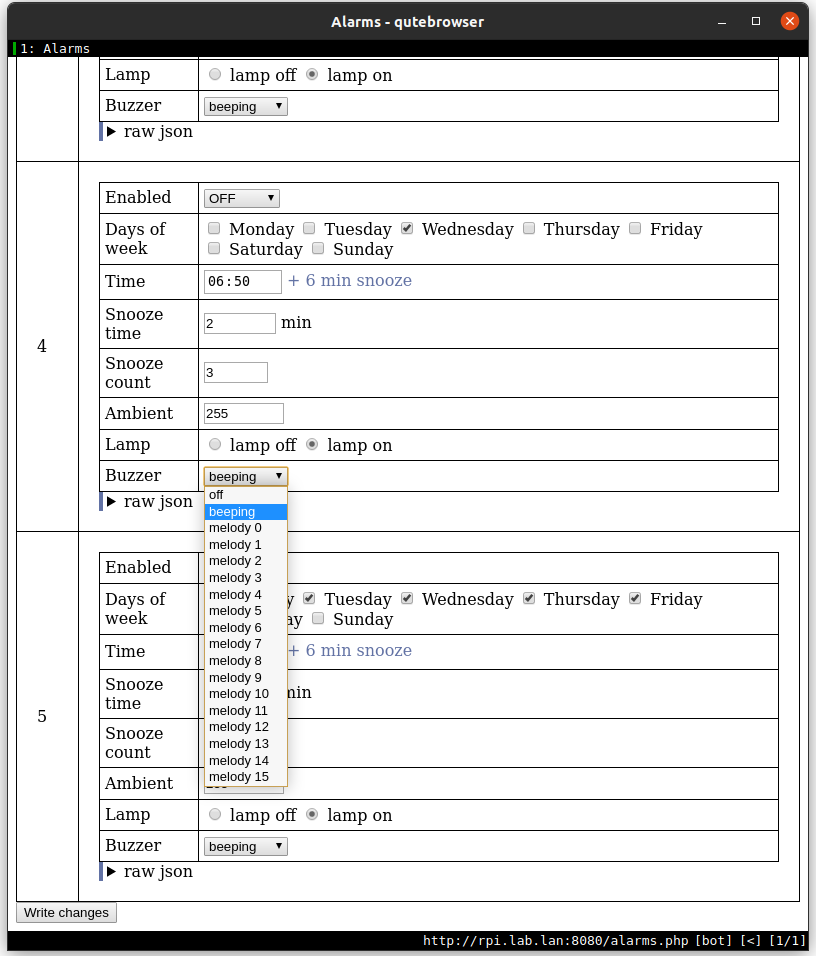
\includegraphics[width=1.00\textwidth]{web-qutebrowser}
    \caption{%
        Webová stránka AlarmClockWeb zobrazená ve webovém prohlížeči
        \shellcmd{qutebrowser}
    }
    \label{fig:web qutebrowser}
\end{figure}

Webová stránka je z hlediska využitých technologií velice jednoduchá, například
vůbec nevyžaduje JavaScript pro základní funkčnost (JavaScript je ale využíván
pro některé doplňkové funkce). Z tohoto důvodu by měla být kompatibilní
s naprostou většinou webových prohlížečů, včetně zastaralých verzí či textových
prohlížečů pro příkazový řádek (viz obrázek~\vref{fig:web links}).

\begin{figure}[htbp]
    \begin{lstlisting}[style=terminal,columns=fixed]
                                                    Alarms (p1 of 13) 
                             Alarm Clock                              
                                                                      
Alarms                                                                
                                                                      
   This simple UI allows for reading and writing configuration of     
   alarms.                                                            
                                                                      
   +--------------------------------------------------------------+   
   | Index | Configuration                                        |   
   |-------+------------------------------------------------------|   
   |       | +--------------------------------------------------+ |   
   |       | | Enabled      | [+---------+                      | |   
   |       | |--------------+--| unknown |----------------------| |   
   |       | |              | [| OFF     | ] Tuesday [ ]        | |   
   |       | | Days of week | W| SGL     |] Thursday [X] Friday | |   
   |       | |              | [| RPT     | [ ] Sunday           | |   
   |       | |--------------+--| SKP     |----------------------| |   
   |       | | Time         | 1+---------+_________             | |   
   |       | |--------------+-----------------------------------| |   
   |       | | Snooze time  | 1____________________  min        | |   
   |       | |--------------+-----------------------------------| |   
   |       | | Snooze count | 1____________________             | |   
Select field, name a0-enabled                                        
    \end{lstlisting}
    {\footnotesize (Menu \uv{Enabled} je rozbalené. Ve skutečném terminálu je
    vybraná položka zvýrazněna prohozením barvy pozadí a popředí.)}
    \caption{AlarmClockWeb v terminálovém webovém prohlížeči \shellcmd{links}}
    \label{fig:web links}
\end{figure}

\todo[inline]{MQTT knihovna a jednoduchy priklad?}

Použitá knihovna \texttt{php-mqtt/client} vyžaduje PHP verze 7.4. Operační
systém Debian 10 (buster) ale nabízí ve standardních repozitářích pouze PHP
7.3. Existuje možnost doinstalovat balíčky třetích stran, to by ale mohlo
způsobit problémy s ostatními službami běžícími na stejném systému (pokud
potřebují PHP 7.3 a s PHP 7.4 nefungují).
U programů napsaných v jazyce Python (jako například MQTT adaptér) je řešení
podobných problémů velice jednoduché, protože můžeme využít virtuální prostředí
\texttt{virtualenv}. Pro PHP spouštěné webových serverem Apache ale žádné
podobné řešení neexistuje.
Proto byl vytvořen soubor \filename{Dockerfile}, který obsahuje definici
kontejneru. V tomto kontejneru běží zcela oddělená instance Apache s vlastní
konfigurací a vlastní verzí PHP. To přináší i další výhody. Protože služba běží
ve velice dobře definovaném prostředí, které je na všech systémech stejné,
snižuje se například riziko výskytu chyb vyplývajících z konfigurace
webserveru. Jako základ je použit kontejner \texttt{php:7.4-apache}, do kterého
je doinstalován program pro instalaci PHP knihoven \shellcmd{composer}
a nakopírovány zdrojové kódy AlarmClockWeb.
\lstinputlisting[language=Dockerfile,style=numbers]{prilohy/AlarmClockWeb/Dockerfile}
Pořadí příkazů v \filename{Dockerfile} je důležité. Nejde jen o běžné požadavky
(například soubor musí být do kontejneru nakopírován před tím, než jej můžeme
číst). Každá instrukce \texttt{RUN}, \texttt{COPY} či \texttt{ADD} vytváří
novou vrstvu. Jednotlivé vrstvy jsou drženy v mezipaměti a drobná změna ve
zdrojových kódech naší webové aplikaci proto nemusí znamenat sestavení celého
obrazu od úplného počátku. Z tohoto důvodu je vhodné postavit
\filename{Dockerfile} tak, aby pouhá změna v jednom ze zdrojových souborů
aplikace nevedla k invalidaci celé mezipaměti. Tato změna totiž vyžaduje pouze
nakopírování nového souboru do obrazu kontejneru, není ale třeba například
znovu instalovat všechny softwarové balíčky.

\shellcmd{docker} umožňuje distribuci již sestavených obrazů, například na
webovém portálu Docker Hub. Pro tento malý projekt s minimem uživatelů ale
udržování vlastní binární distribuce a řešení bezpečnostních problémů s tím
spojených není výhodné.


Nasazení služby AlarmClockWeb na linuxový server se zjednodušuje na několik
příkazů:
\begin{lstlisting}[language=mybash,style=numbers]
# Zkopírujeme ukázkovou konfiguraci do config.php
cp config-sample.php config.php
# Nyní je potřeba konfiguraci upravit a správně nastavit
# např. adresu MQTT # brokeru.

# Sestavíme obraz kontejneru z instrukcí v Dockerfile.
docker build -t alarmclockweb .

# Spustíme vlastní kontejner.
# Soubor config.php v aktuální složce ($PWD) je připojen ke kontejneru.
# Pokud již na portu 80 poslouchá jiná služba,
# můžeme použít například -p 8080:80.
docker run -d \
    --name alarmclockweb \
    -p 80:80 \
    -v $PWD/config.php:/var/www/html/config.php:ro \
    alarmclockweb
\end{lstlisting}

Pokud je požadována integrace se složitější webovou stránkou, lze v konfiguraci
jejího webového serveru nastavit funkci reverzní proxy. Tímto způsobem lze
i přidat dodatečné funkce, jako například ověřování uživatelských hesel.
Následuje příklad konfigurace webového serveru Apache.
Předpokladem je, že kontejner \texttt{alarmclockweb} vystavuje port
\port{8080}. Pro zamezení přímého připojení uživatele na port \port{8080}
serveru je vhodné specifikovat při spouštění kontejneru argument
\texttt{-p 127.0.0.1:8080:80}, kterým je připojení na port \port{8080} omezeno
na rozhraní \texttt{loopback} s IP adresou \ipaddress{127.0.0.1}.
\begin{lstlisting}[style=numbers]
# alarmclockweb docker container
<Location /alarmclock>
        AuthType Basic
        AuthName "AlarmClockWeb"
        AuthBasicProvider file
        # htpasswd -c /etc/apache2/.htpasswd uzivatel
        AuthUserFile /etc/apache2/.htpasswd
        Require user uzivatel
</Location>
ProxyPass /alarmclock http://localhost:8080/
ProxyPassReverse /alarmclock http://localhost:8080/
\end{lstlisting}
